\chapter{Training}

Seguono le immagini dei risultati. Osservazioni:
\begin{itemize}
    \item Il numero di EPOCHS di alcuni risultati è dettata da fattori "arbitrari". Ad esempio il learning rate di alcuni training è stato settato molto piccolo, dunque il tempo di training è più lungo. Questo è stato fatto principalmente per evitare un bug (che ho già accennato a Christian e che anche lui ha già avuto...) di matrici che NON dipende da me...
    \item Non conosco precisamente il significato del lr (learning rate) nello specifico nell'optimizer usato (Adam)
    \item Non conosco precisamente come scegliere l'optimizer. Quello impostato è di default; è possibile cambiarlo e ho intenzione di valutare quale (tra quelli già in gpytorch...) è da preferire
    \item Non conosco precisamente il funzionamento dell'EarlyStopper, programmato da Stefano Longobardi. Non conosco precisamente il funzionamento di alpha (parametro per l'EarlyStopper) né il funzionamento di patience (altro parametro di EarlyStopper)
    \item Non ho implementato la ripetizione del training per velocizzare la generazione delle immagini e inserirle con facilità nel capitolo "temporaneo". Ovviamente in sede di "bella copia" le implementerò, cosa che permetterà all'emulatore di selezionare il "migliore" training.
    \item Lo strano comportamento del grafici MAP - Pd, SBP - Pd, DBP - Pd, PP - Pd (in realtà abbastanza preciso guardando la scala...) non so bene come giustificarlo... Sono abbastanza sicuro che dipenda dalla bassa sensitività locale, cioè dal fatto che infici molto poco nell'output.
    \item Si noti che i risultati si possono migliorare aumentando la mole del dataset, tenuto abbastanza piccolo per rimanere in tempi veloci per facilitare la stesura di questo capitolo temporaneo... Potrebbe essere oggetto di studio anche la dimensione del dataset per ottenere risultati precisi (imponendosi una tolleranza), ma credo abbia senso farla dopo lo studio delle singole componenti di ML usate dall'API 
    \item Ci sono early stopper che "non hanno funzionato", cioè il training ha finito al numero massimo di EPOCHS impostato. Questo dipende da una componente randomica nello starting del training: a volte un certo early stopper funziona in un certo modo (termina ad una certa EPOCH) altre volte in un altro modo; questo complica la scelta dei parametri dell'early stopper
\end{itemize}

%%%%%%%%%%%%%%%%%%%%%%%%%%%%%
%%%%%%%%%%%%%%%%%%%%%%%%%%%%%
%             MAP
%%%%%%%%%%%%%%%%%%%%5%%%%%%%%%
%%%%%%%%%%%%%%%%%%%%%%%%%%%%
\newpage

\section{MAP}
\begin{figure}[h]
    \centering
    \includegraphics[width=1\textwidth]{images/Training - temp/MAP - dataset.png}
    \caption{Dataset (lo ometto successivamente perché uguale)}
\end{figure}

\newpage

\begin{figure}[h]
    \centering
    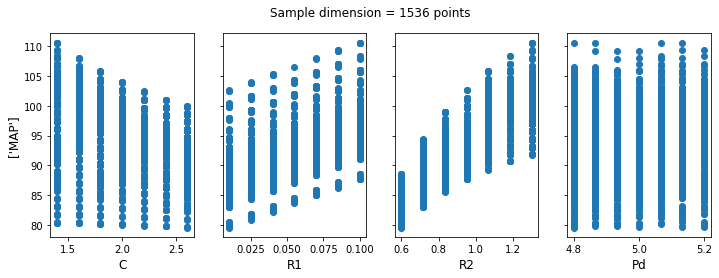
\includegraphics[width=1\textwidth]{images/Training - temp/MAP - parametri.png}
    \caption{Plot: MAP vs single parameter. Sotto vengono riproposti i singoli grafici fatti meglio.}
\end{figure}

\newpage

\begin{figure}[h]
    \centering
    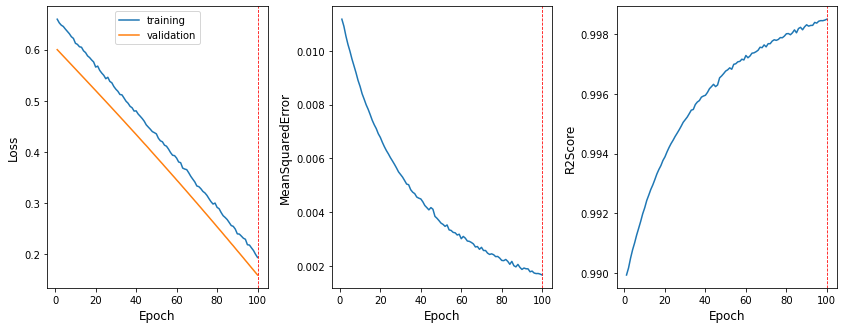
\includegraphics[width=1\textwidth]{images/Training - temp/MAP - loss.png}
    \caption{Loss, no early stopper, 100 EPOCHS}
\end{figure}

\newpage

\begin{figure}[h]
    \centering
    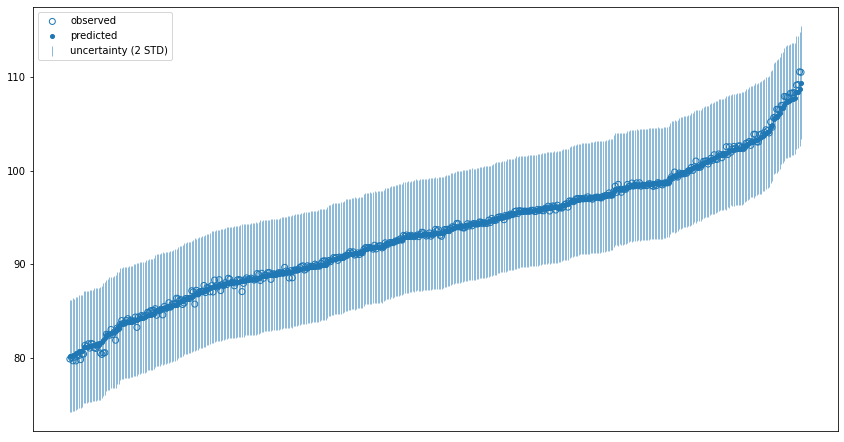
\includegraphics[width=1\textwidth]{images/Training - temp/MAP - inference.png}
    \caption{Inference, no early stopper, 100 EPOCHS}
\end{figure}

\newpage

\begin{figure}[h]
    \centering
    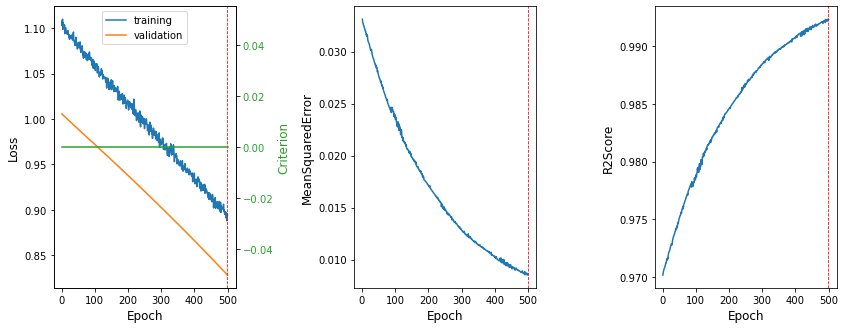
\includegraphics[width=1\textwidth]{images/Training - temp/MAP - loss - early stopper.png}
    \caption{Loss, early stopper. Ho riscontrato il bug per cui ho dovuto diminuire di molto il lr, dunque ha richiesto molti più EPOCH di quanto (se non avviene tale bug) si possa raggiungere.}
\end{figure}

\newpage

\begin{figure}[h]
    \centering
    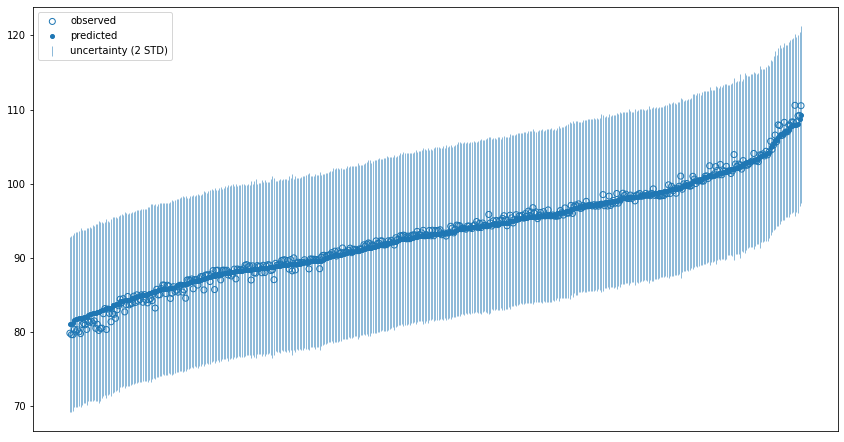
\includegraphics[width=1\textwidth]{images/Training - temp/MAP - inference - early stopper.png}
    \caption{Inference, early stopper.}
\end{figure}

\newpage
Seguono quattro grafici: MAP - C, R1, R2, Pd. Per farli ho generato un dataset (diverso da quello per il training) con solo un parametro in input che variasse, mentre gli altri restavano fissi. (Quindi per MAP - C ho generato un dataset in cui R1, R2 e PD sono fissi e C varia) Ho predetto per ogni entry del dataset la MAP e l'ho controntata con quella che calcolo col Windkessel.


\begin{figure}[h]
    \centering
    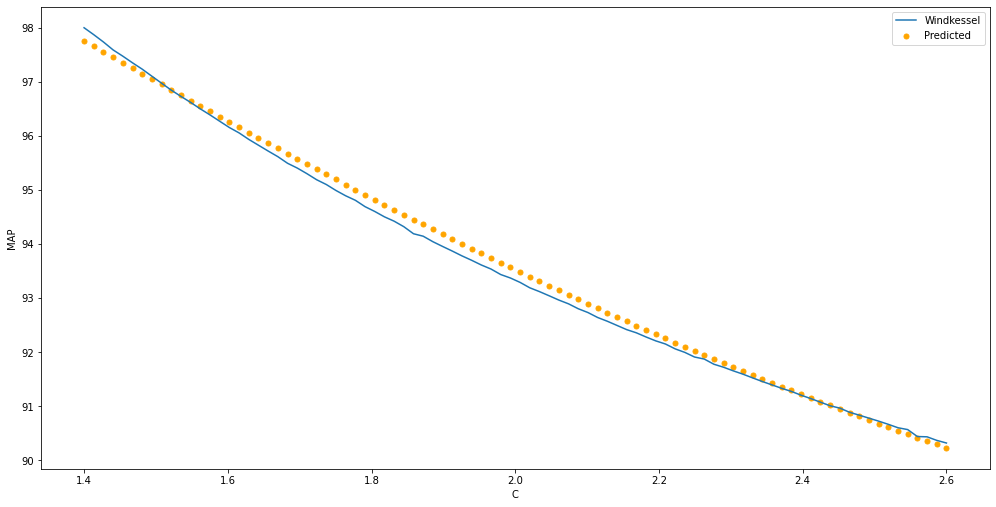
\includegraphics[width=1\textwidth]{images/Training - temp/MAP - C.png}
    \caption{MAP - C}
\end{figure}

\newpage

\begin{figure}[h]
    \centering
    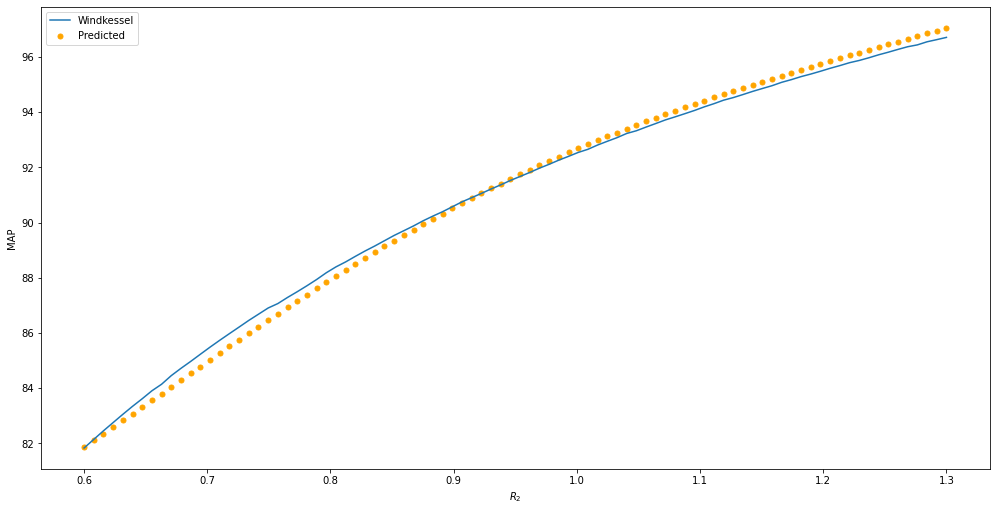
\includegraphics[width=1\textwidth]{images/Training - temp/MAP - R2.png}
    \caption{MAP - R2}
\end{figure}

\newpage

\begin{figure}[h]
    \centering
    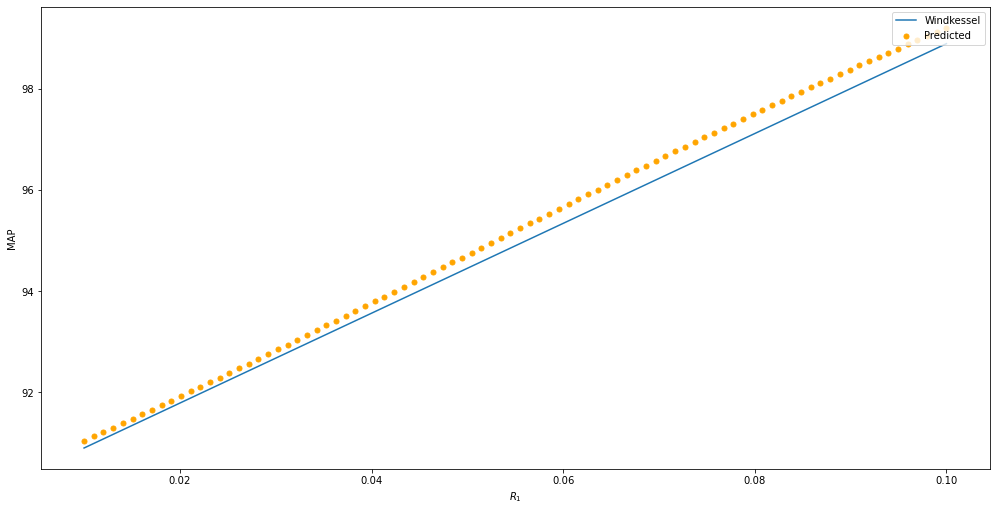
\includegraphics[width=1\textwidth]{images/Training - temp/MAP _ R1.png}
    \caption{MAP - R1}
\end{figure}

\newpage


\begin{figure}[h]
    \centering
    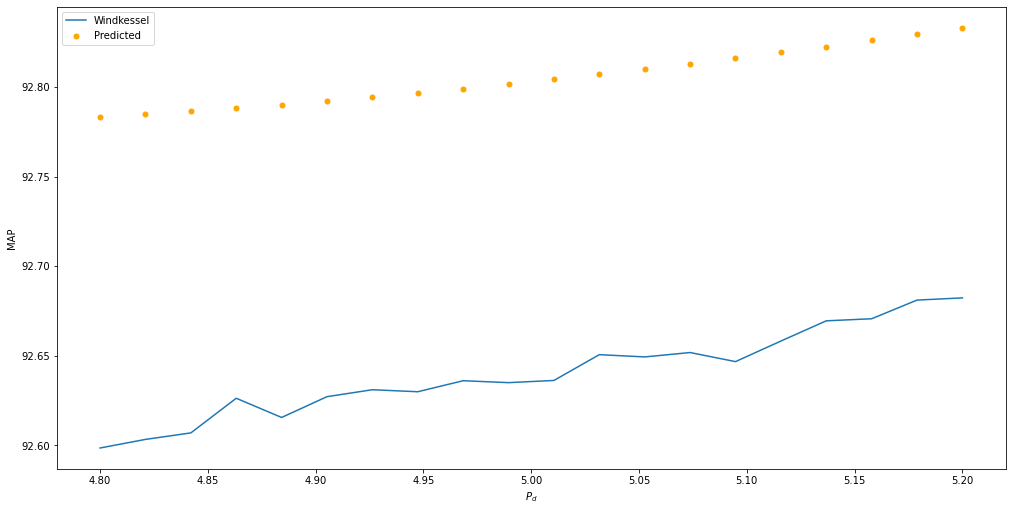
\includegraphics[width=1\textwidth]{images/Training - temp/MAP - Pd.png}
    \caption{MAP - Pd}
\end{figure}

%%%%%%%%%%%%%%%%%%%%%%%%%%%%%
%%%%%%%%%%%%%%%%%%%%%%%%%%%%%
%             DBP
%%%%%%%%%%%%%%%%%%%%5%%%%%%%%%
%%%%%%%%%%%%%%%%%%%%%%%%%%%%
\newpage
\section{DBP}

\begin{figure}[h]
    \centering
    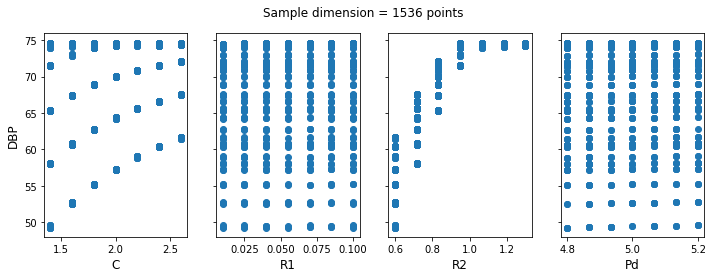
\includegraphics[width=1\textwidth]{images/Training - temp/DBP - parameters.png}
    \caption{DBP - parameters (meglio sotto)}
\end{figure}

\newpage


\begin{figure}[h]
    \centering
    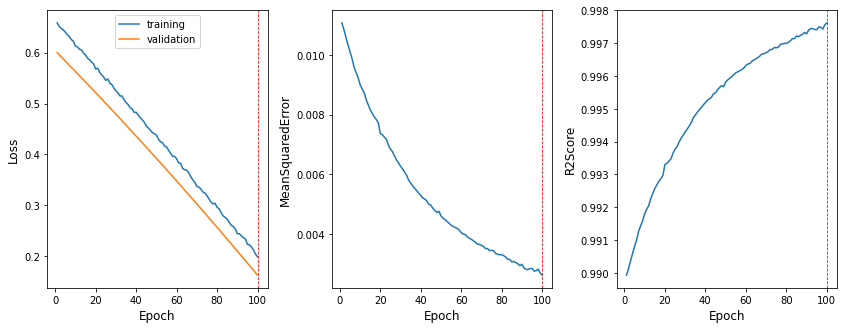
\includegraphics[width=1\textwidth]{images/Training - temp/DBP - loss.png}
    \caption{Loss, no early stopper, 100 EPOCHS}
\end{figure}


\newpage


\begin{figure}[h]
    \centering
    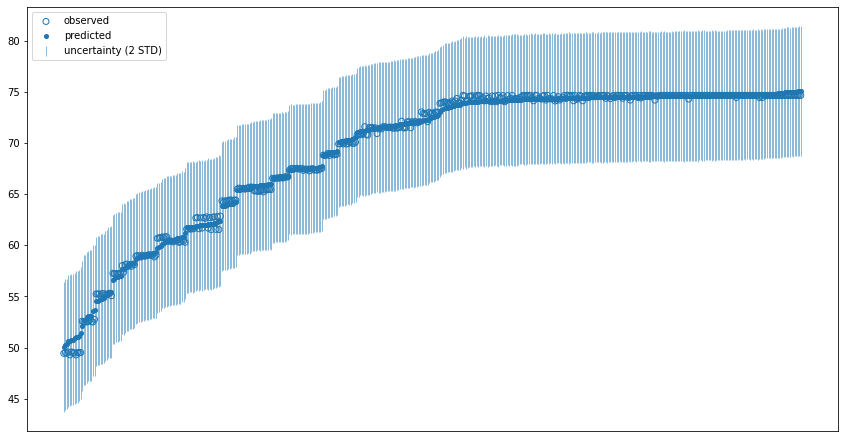
\includegraphics[width=1\textwidth]{images/Training - temp/DBP - inference.png}
    \caption{Inference, no early stopper, 100 EPOCHS}
\end{figure}



\newpage


\begin{figure}[h]
    \centering
    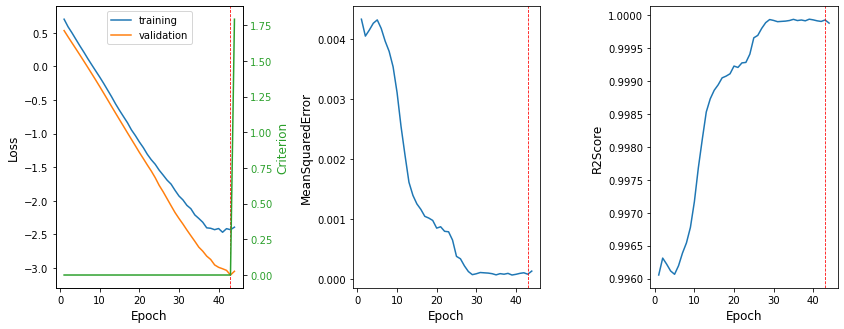
\includegraphics[width=1\textwidth]{images/Training - temp/DBP - loss - early stopper.png}
    \caption{Loss, early stopper (non ho riscontrato bug, l'early stopper ha funzionato bene in questo caso. Si noti che è stato cambiato anche il lr, cosa che, in combinazione con l'early stopper, ha ridotto notevolmente il numero di EPOCHS.)}
\end{figure}


\newpage


\begin{figure}[h]
    \centering
    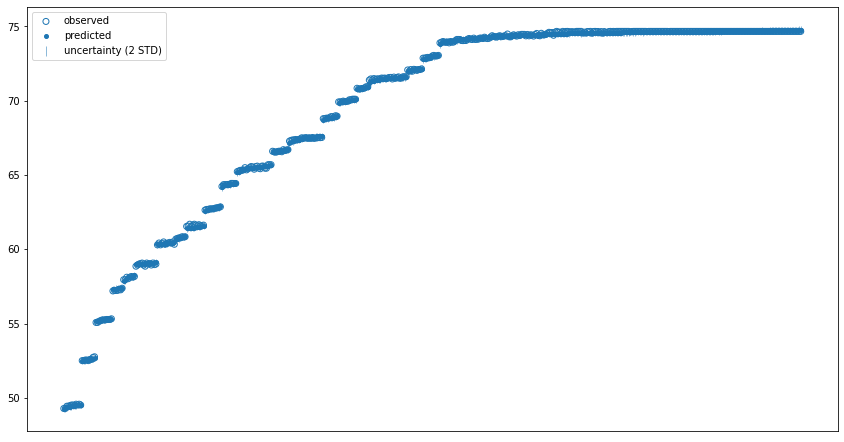
\includegraphics[width=1\textwidth]{images/Training - temp/DBP - inference - early stopper.png}
    \caption{Inference, early stopper}
\end{figure}


\newpage
Non sono sicuro se ciò che segue sia colpa mia (codice sbagliato) oppure no. In parte ha senso: il RBF kernel genera funzioni $C^\infty$; mi aspetto che con un altro kernel si raggiunga una maggiore precisione. Ad esempio per DBP - C un linear kernel potrebbe forse fare di meglio...

\begin{figure}[h]
    \centering
    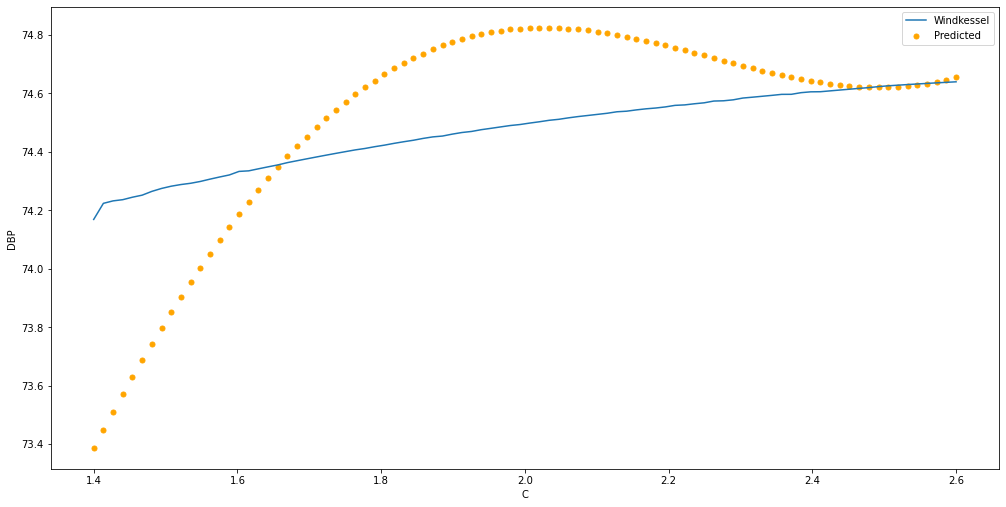
\includegraphics[width=1\textwidth]{images/Training - temp/DBP - C.png}
    \caption{DBP - C}
\end{figure}

\newpage


\begin{figure}[h]
    \centering
    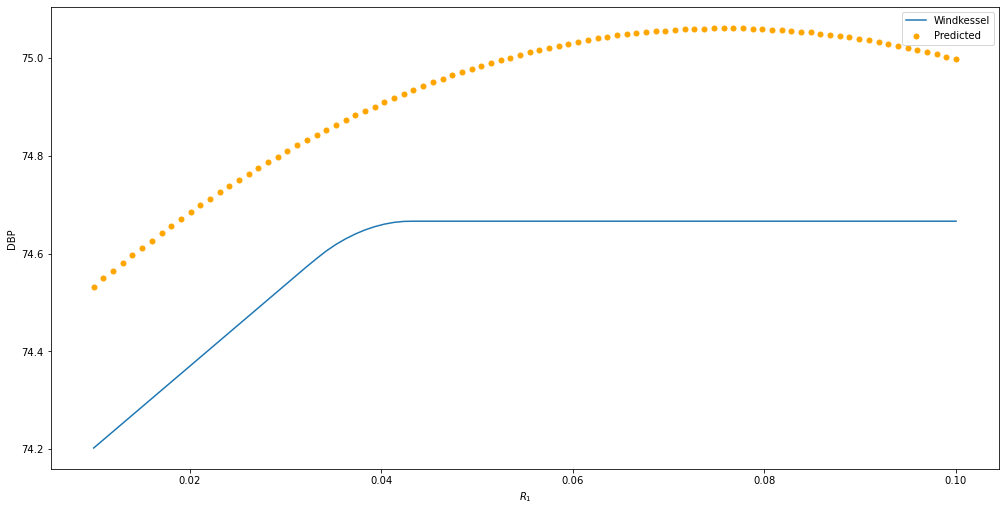
\includegraphics[width=1\textwidth]{images/Training - temp/DBP - R1.png}
    \caption{DBP - R1}
\end{figure}

\newpage


\begin{figure}[h]
    \centering
    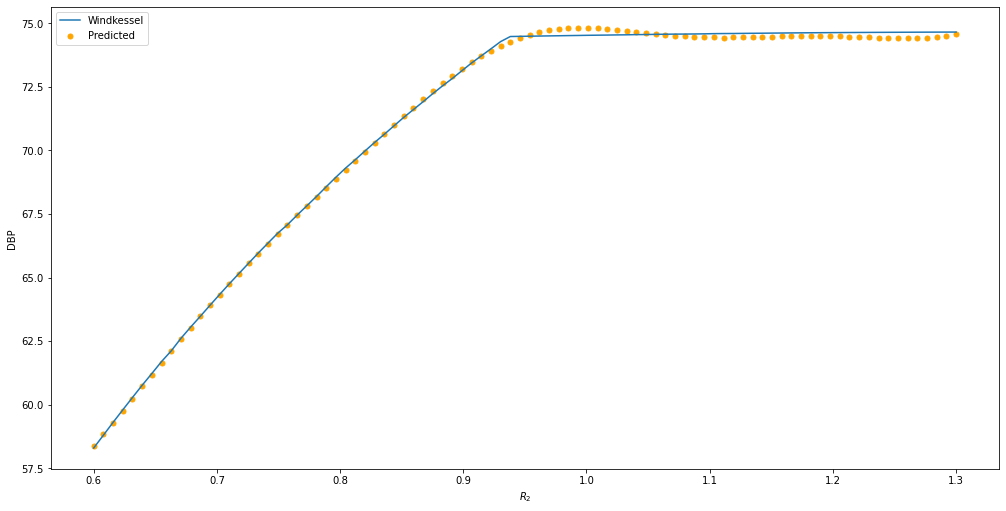
\includegraphics[width=1\textwidth]{images/Training - temp/DBP - R2.png}
    \caption{DBP - R2}
\end{figure}

\newpage


\begin{figure}[h]
    \centering
    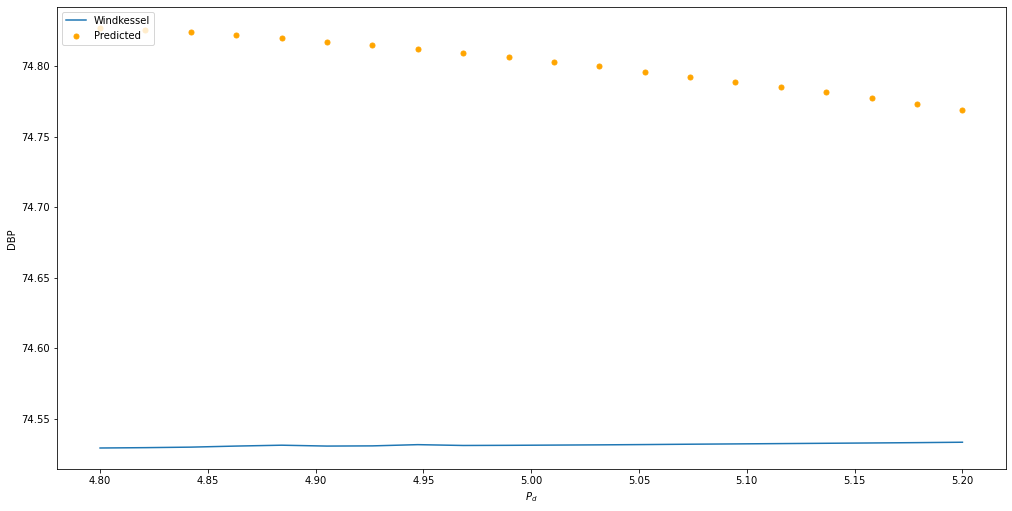
\includegraphics[width=1\textwidth]{images/Training - temp/DBP - Pd.png}
    \caption{DBP - Pd}
\end{figure}






%%%%%%%%%%%%%%%%%%%%%%%%%%%%%
%%%%%%%%%%%%%%%%%%%%%%%%%%%%%
%             SBP
%%%%%%%%%%%%%%%%%%%%5%%%%%%%%%
%%%%%%%%%%%%%%%%%%%%%%%%%%%%
\newpage
\section{SBP}
\begin{figure}[h]
    \centering
    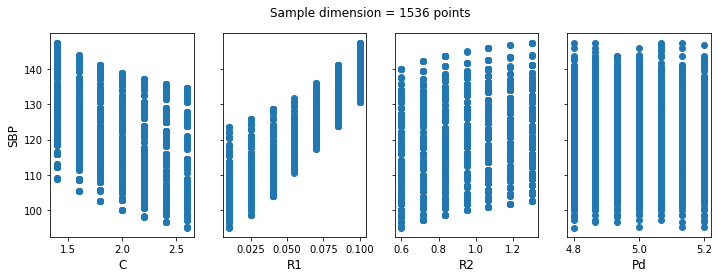
\includegraphics[width=1\textwidth]{images/Training - temp/SBP - parameters.png}
    \caption{SBP - parameters (meglio sotto)}
\end{figure}

\newpage

\begin{figure}[h]
    \centering
    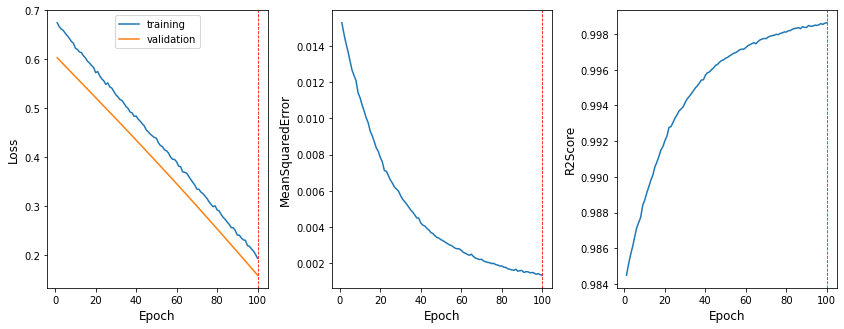
\includegraphics[width=1\textwidth]{images/Training - temp/SBP - loss.png}
    \caption{Loss, no early stopper, 100 EPOCHS}
\end{figure}


\newpage

\begin{figure}[h]
    \centering
    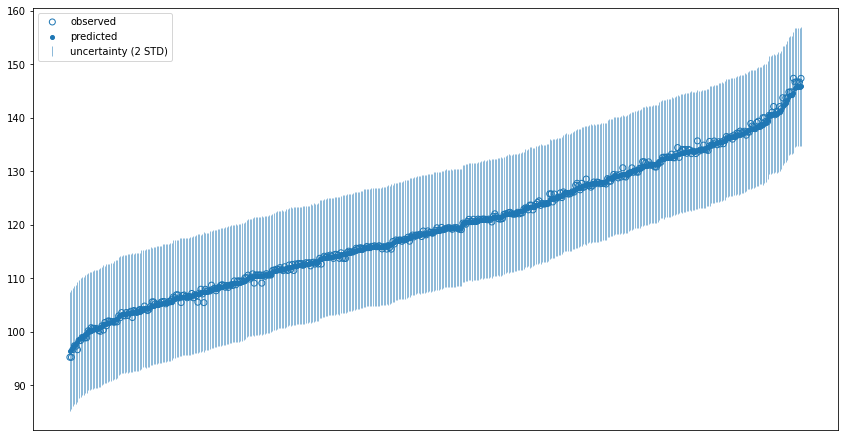
\includegraphics[width=1\textwidth]{images/Training - temp/SBP - inference.png}
    \caption{Inference, no early stopper, 100 EPOCHS}
\end{figure}


\newpage

\begin{figure}[h]
    \centering
    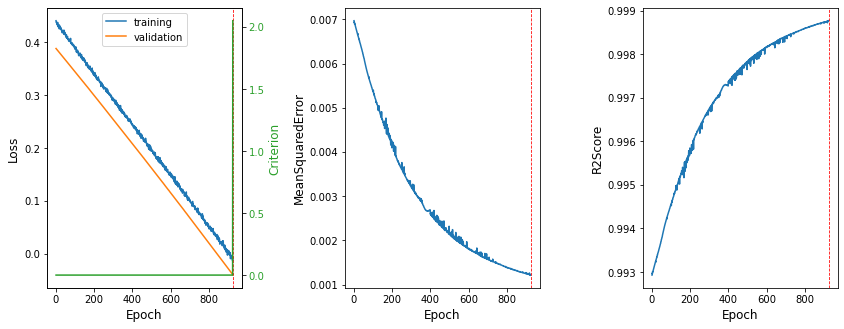
\includegraphics[width=1\textwidth]{images/Training - temp/SBP - loss - early stopper.png}
    \caption{Loss, early stopper (Early stopper ha funzionato, penso si possa fare di meglio conoscendone bene il funzionamento...)}
\end{figure}


\newpage

\begin{figure}[h]
    \centering
    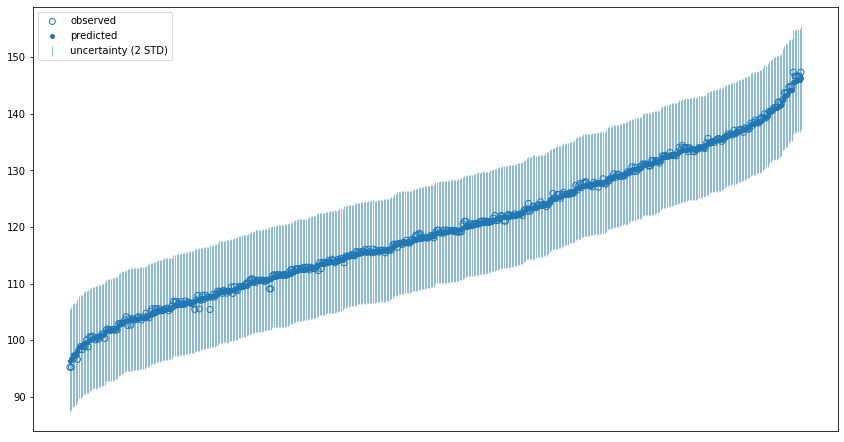
\includegraphics[width=1\textwidth]{images/Training - temp/SBP - inference - early stopper.png}
    \caption{Inference, early stopper}
\end{figure}

\newpage

\begin{figure}[h]
    \centering
    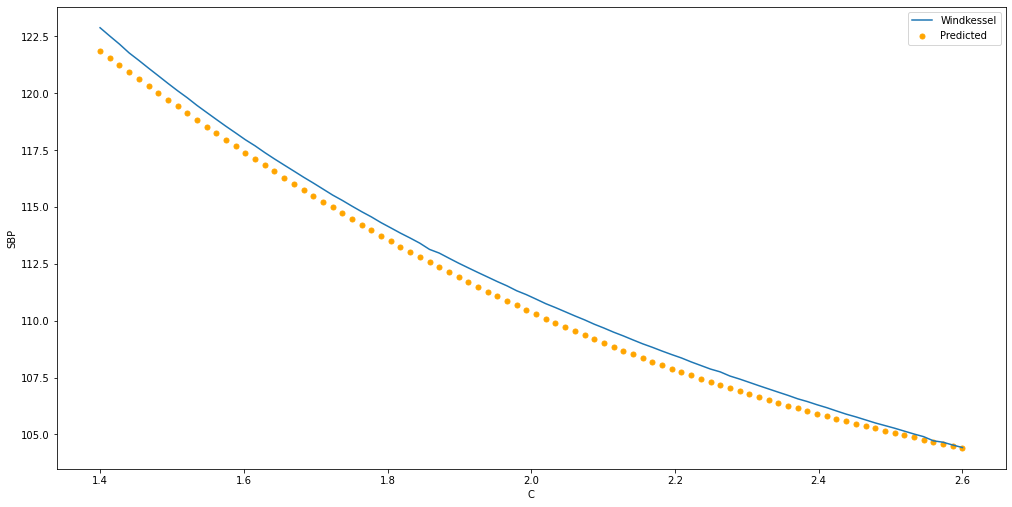
\includegraphics[width=1\textwidth]{images/Training - temp/SBP - C.png}
    \caption{SBP - C}
\end{figure}

\newpage

\begin{figure}[h]
    \centering
    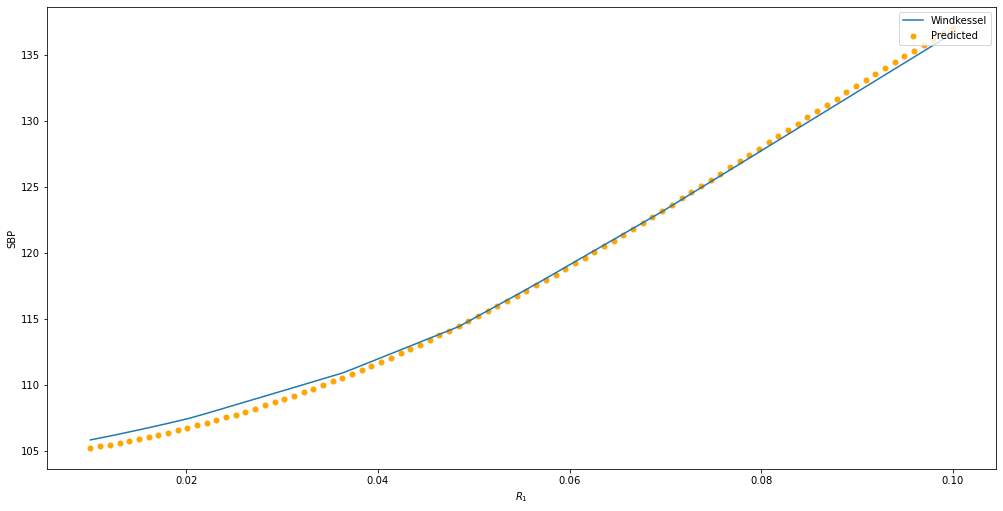
\includegraphics[width=1\textwidth]{images/Training - temp/SBP - R1.png}
    \caption{SBP - R1}
\end{figure}


\newpage

\begin{figure}[h]
    \centering
    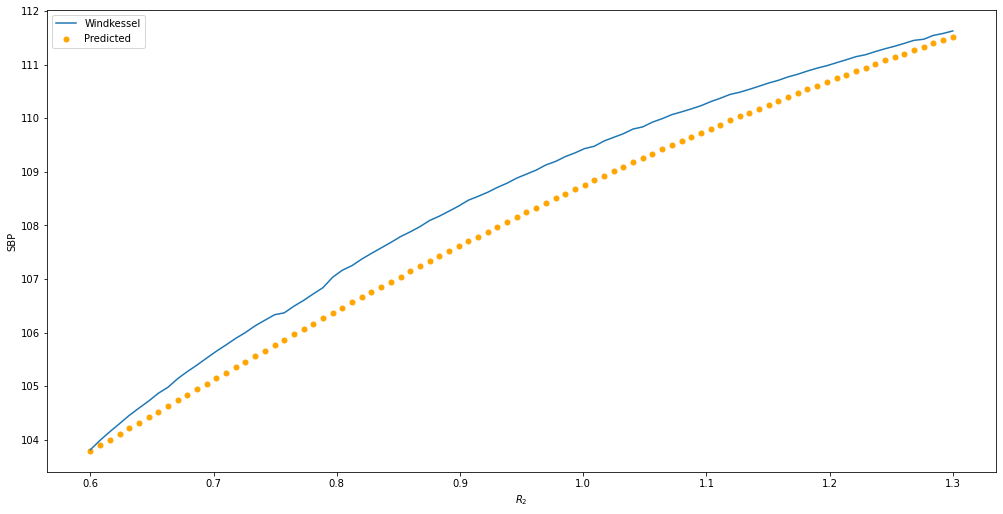
\includegraphics[width=1\textwidth]{images/Training - temp/SBP - R2.png}
    \caption{SBP - R2}
\end{figure}


\newpage

\begin{figure}[h]
    \centering
    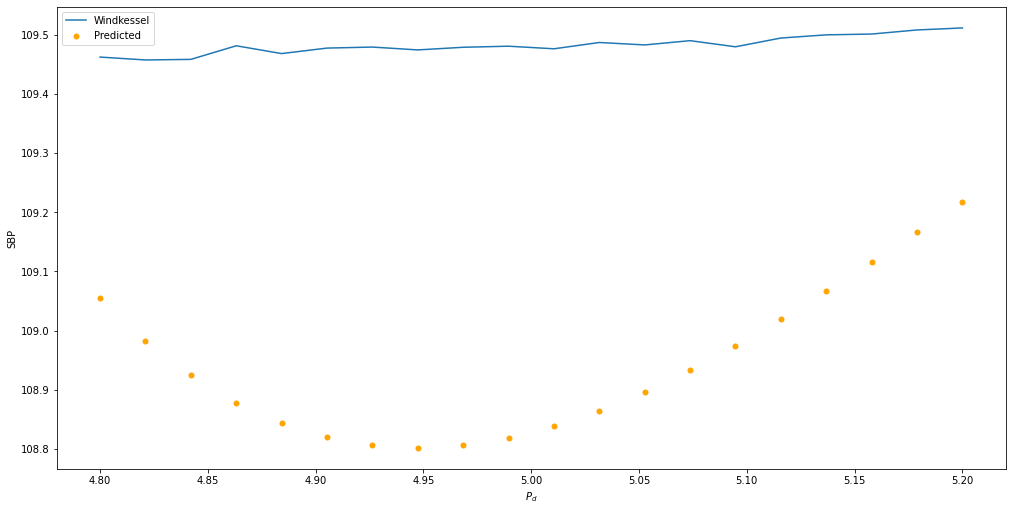
\includegraphics[width=1\textwidth]{images/Training - temp/SBP - Pd.png}
    \caption{SBP - Pd}
\end{figure}










%%%%%%%%%%%%%%%%%%%%%%%%%%%%%
%%%%%%%%%%%%%%%%%%%%%%%%%%%%%
%             PP
%%%%%%%%%%%%%%%%%%%%5%%%%%%%%%
%%%%%%%%%%%%%%%%%%%%%%%%%%%%
\newpage
\section{PP}

\begin{figure}[h]
    \centering
    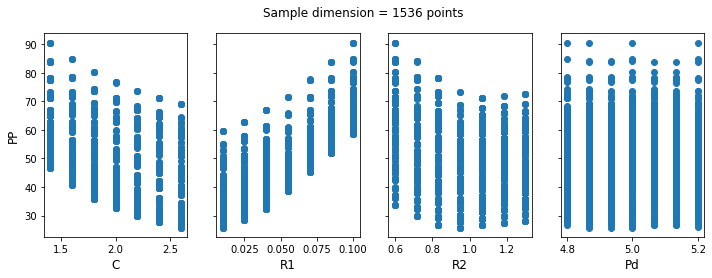
\includegraphics[width=1\textwidth]{images/Training - temp/PP - parametri.png}
    \caption{PP - parametri (meglio sotto)}
\end{figure}


\newpage


\begin{figure}[h]
    \centering
    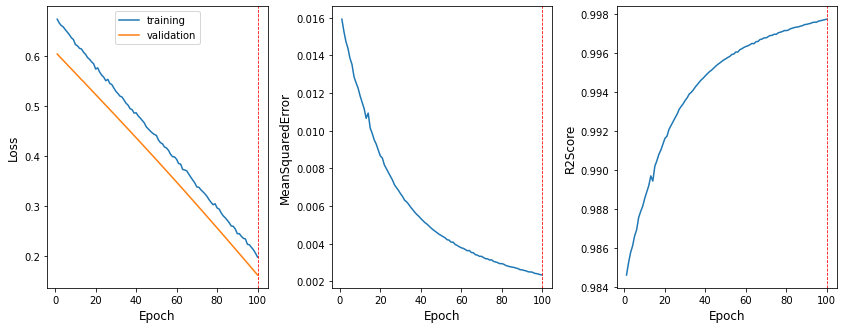
\includegraphics[width=1\textwidth]{images/Training - temp/PP - loss.png}
    \caption{Loss, no early stopper, 100 EPOCHS}
\end{figure}



\newpage
\begin{figure}[h]
    \centering
    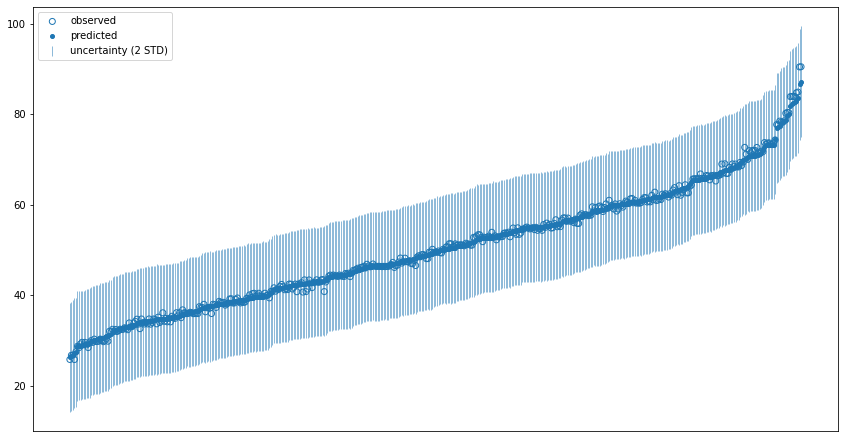
\includegraphics[width=1\textwidth]{images/Training - temp/PP - inference.png}
    \caption{Inference, no early stopper, 100 EPOCHS}
\end{figure}


\newpage
\begin{figure}[h]
    \centering
    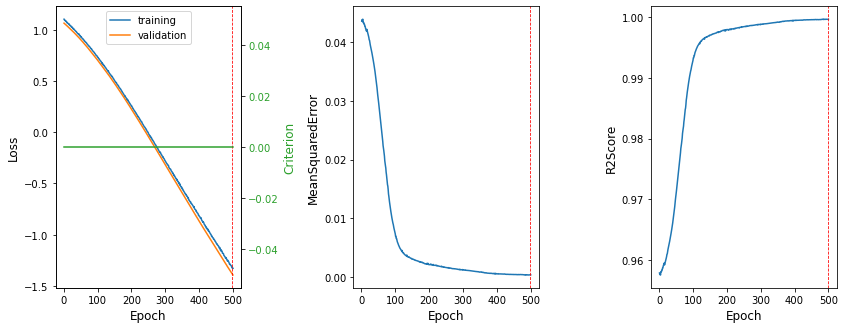
\includegraphics[width=1\textwidth]{images/Training - temp/PP - loss - early inference.png}
    \caption{Loss, early stopper (l'early stopper non ha funzionato e ha finito al massimo delle EPOCHS impostate)}
\end{figure}



\newpage
\begin{figure}[h]
    \centering
    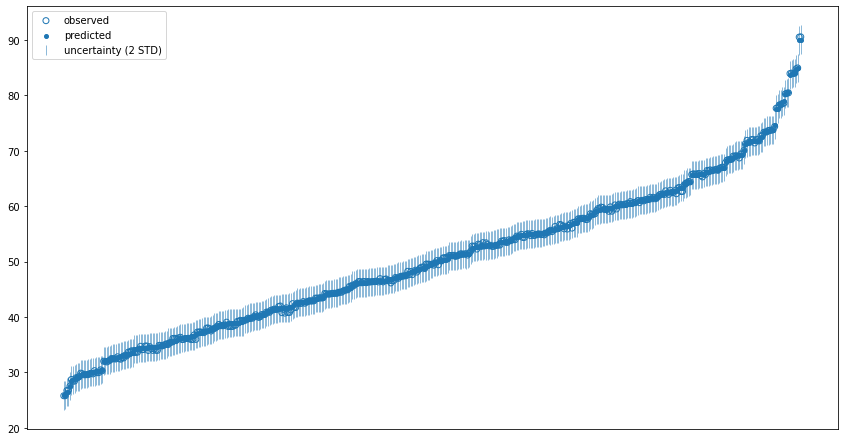
\includegraphics[width=1\textwidth]{images/Training - temp/PP - inference - early stopper.png}
    \caption{Inference, early stopper}
\end{figure}


\newpage
\begin{figure}[h]
    \centering
    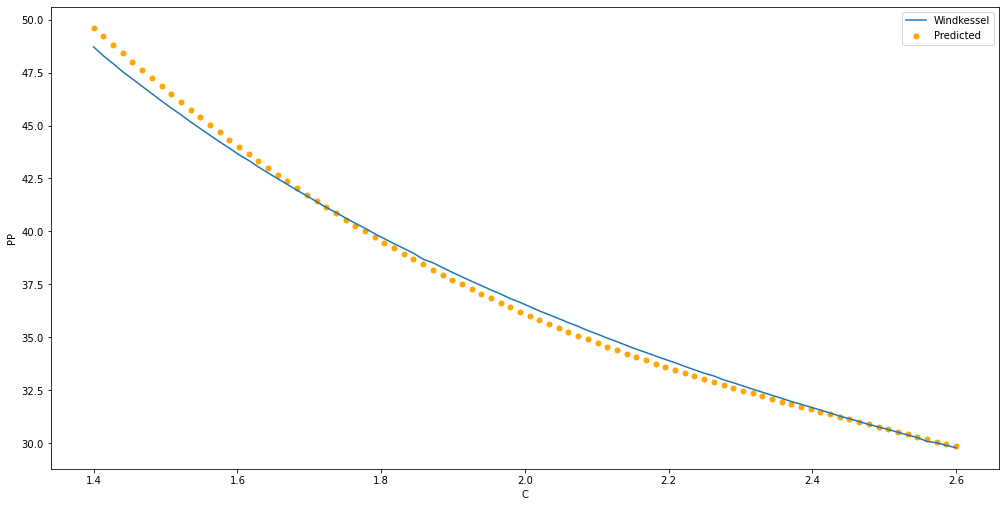
\includegraphics[width=1\textwidth]{images/Training - temp/PP - C.png}
    \caption{PP - C}
\end{figure}


\newpage
\begin{figure}[h]
    \centering
    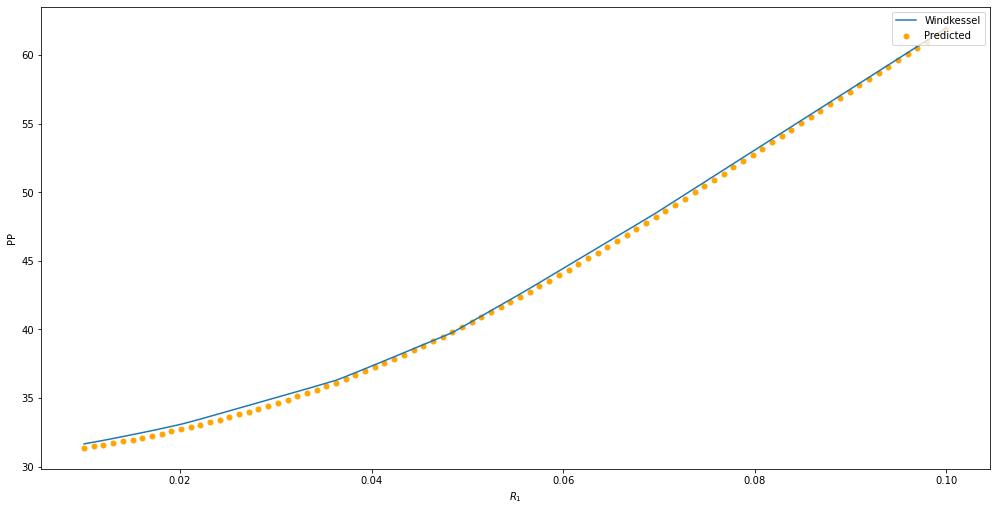
\includegraphics[width=1\textwidth]{images/Training - temp/PP - R1.png}
    \caption{PP - R1}
\end{figure}

\newpage
\begin{figure}[h]
    \centering
    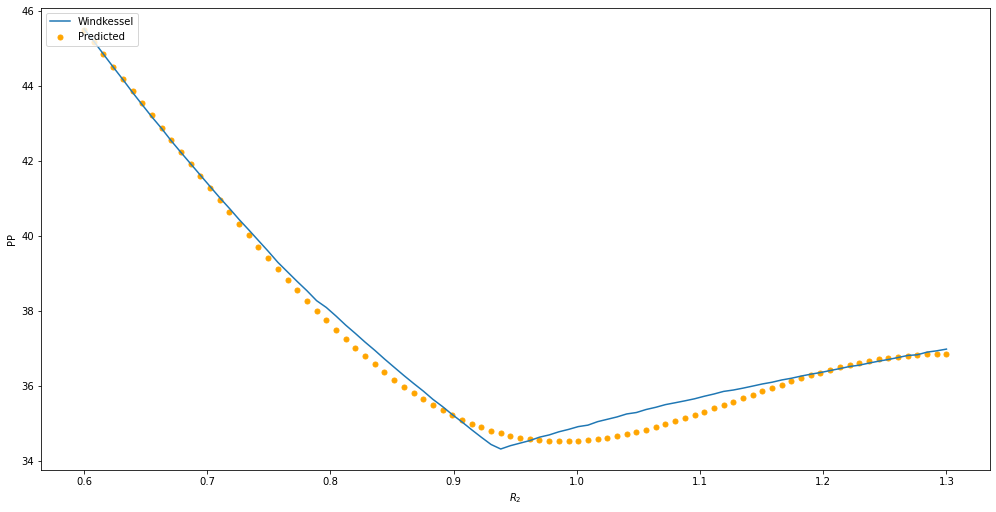
\includegraphics[width=1\textwidth]{images/Training - temp/PP - R2.png}
    \caption{PP - R2}
\end{figure}

\newpage
\begin{figure}[h]
    \centering
    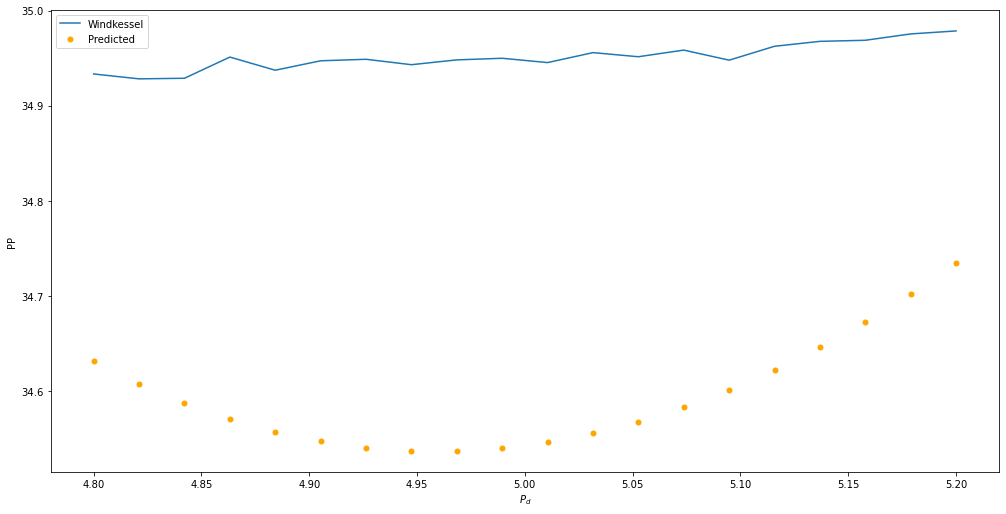
\includegraphics[width=1\textwidth]{images/Training - temp/PP - Pd.png}
    \caption{PP - Pd}
\end{figure}


















\newpage
Possibili future directions:
\begin{itemize}
    \item Comprendere e scegliere bene l'EarlyStopper. Dovrebbero essercene anche di già implementati (preferibili, a mio avviso) e esplorerò questo mondo
    \item Comprendere e scegliere il preferito optimizer (quello che ora è Adam) e relativi parametri
    \item Usare un external validation set potrebbe aumentare la precisione. Se avessimo un dataset "reale" (diversi pazienti veri) si potrebbe forse addirittura ottenere dei risultati che superino la precisione del modello Windkessel (not sure...). Mi rendo conto richieda del tempo però e non so se esistano database simili...
    \item Scegliere altre (migliori?) loss function case-specific
    \item Rifare il training senza Pd in input e confrontare i risultati (oppure decidere proprio di toglierla...)
    \item Provare a settare il dataset in modo da migliorare i risultati (variabile) - (parametro), magari impostando come validation set combinazioni di parametri realistiche, fingendo quindi che siano misurati su pazienti; per il training e testing usare combinazioni di dati più estreme e meno realistiche. Non so se possa funzionare...
\end{itemize}

Queste direzioni future peraltro rientrano nei possibili interessi di Christian e potrebbero essere "facilmente" adattate al suo modello. (mi riferisco soprattutto alla scelta dell'optimizer, del lr, dell'EarlyStopper, della scelta del Kernel)\\

Per ora il K-fold cross validation mi sembra "secondario": prima sistemerei i problemi / dubbi su questo tipo di training, poi mi sposterei sulle K-fold cross validation... 